\section{Software Development}
\label{sec:softwareDevelopment}
  Previously mentioned was the manner in which the software design and development workflow differed from those of the mechanical and electrical systems as well as the fact that the software system design was driven by the mechanical design and engineering choices therein. For these reasons, many structural and functional design and development choices in the software system were made after the design. This section briefly covers those design choices as well as describes the environment in which the software was developed and deployed.
    
  \subsection{Development Environment}
    \subsubsection{Project Structures}
      The three software components' development projects were kept as similar in structure as possible, which was achievable due to the use of JavaScript for all of them, two of which were Node.js applications. The file VCS used for the projects was Git with the forward looking intention of deploying the source on GitHub for open source collaboration. The common structure included the git-related files and the \mintinline{text}{package.json} file, a file used to describe the project for tools that required such information such as \mintinline{js}{npm} as discussed further on. In the case of the RSVP Client, another metadata file, \mintinline{js}{bower.json} was included as this file listed web module and library dependencies installed using Bower\footnote{Bower: a package management tool used primarily for web-related modules and libraries - \url{https://bower.io/}}. JavaScript source files were placed in a directory off the project root named \mintinline{js}{src}, and utility JavaScript code was placed in the \mintinline{js}{utils} or \mintinline{js}{resources} directory. In the case of the RSVP Client, an additional directory, \mintinline{js}{app}, contained the HTML and Polymer element source to be served to connected Clients.
      
      The RSVP Server and the RCE both required an entry point which was to be invoked by the Node.js runtime. The entry point file, \mintinline{js}{index.js} was placed in the root of the \mintinline{js}{src} directory along with other base level files, such as system sequencers or modules responsible for handling communication. The entry point file also imported the files required by each system, which in turn imported required files and so forth.
      
      Included in each of the projects was a configuration file, either of JSON or JavaScript format, in which static configuration data was stored and read into the software component during execution time. Configuration data included details such as the pin configuration for the PWM extension module or the frequency at which to sample the ADC pins for the proximity sensors. The configuration file made organisation of the data more readable and kept it in one place in the project.
    
    \subsubsection{Build Processes}
      All three of the software components in the software system required some form of build process to ensure that they were suitable for and compatible with the target environments. The \mintinline{text}{package.json} scripts were leveraged for the build processes and scripts were written for cleaning, building and watching (where appropriate). The \mintinline{js}{clean} script cleared out already built files and the \mintinline{js}{build} script performed the necessary steps as part of the build process to generate the required files, placing them in the \mintinline{text}{/build} folder. ``Watching'' invoked the \mintinline{js}{build} script but also indicated to the build tool to rebuild files as they were saved. This also applied to the remote building for the RCE and made the development flow more convenient. The three build processes are described below.
      
      \begin{itemize}
        \item RCE
        \begin{enumerate}
          \item Clean working directory.
          \item Transpile \mintinline{js}{ES6} code to Node.js \mintinline{text}{v6.8.0} compatible JavaScript.
          \item Transmit transpiled code to the RCE board remotely.
        \end{enumerate}
        \item RSVP Server
        \begin{enumerate}
          \item Clean working directory.
          \item Transpile \mintinline{js}{ES6} code to Node.js \mintinline{text}{v7.0.0} compatible JavaScript.
          \item Output transpiled code to the \mintinline{js}{build} folder.
        \end{enumerate}
        \item RSVP Client
        \begin{enumerate}
          \item Clean working directories.
          \item Transpile \mintinline{js}{ES6} Polymer element code into browser compatible JavaScript.
          \item Transpile \mintinline{js}{ES6} source code into browser compatible JavaScript.
          \item Bundle transpiled source code and dependent Node modules into files for browser import.
          \item Output files into the directory accessible by the Server.
        \end{enumerate}
      \end{itemize}
      
    \subsubsection{Project Dependencies}
      Each project made use of multiple open source Node.js modules which were listed in each of the projects' \mintinline{text}{package.json} file. The dependencies are downloaded from remote repositories during the install process provided by the package manager that is bundled in the distribution of Node.js, called \mintinline{js}{npm} (Node.js Package Manager). These packages are listed in Appendix~\ref{appendix:openSourceList} together with a description of each. Towards the end of the project another dependency management tool, \mintinline{js}{yarn}\footnote{Yarn Package Manager - \url{https://github.com/yarnpkg/yarn}}, was used as it provided better caching and faster dependency resolution.
      
    \subsection{Johnny-Five Hardware Abstraction}
      A standard skeletal structure for each of the abstractions written for hardware sub-systems was developed to maintain the consistency of the APIs. Since the \mintinline{js}{edison-io} module, which bridged between the JavaScript \mintinline{js}{mraa} implementation and the J5 \mintinline{js}{Board} instance, was a singleton module, each abstraction file need not have imported a reference to the already existing and running \mintinline{js}{Board}. Snippet~\ref{code:exampleHwAbstractionSkeleton} shows the structure of such an abstraction as well as serves as an example of the general structure of all JavaScript files written for all projects.
      
      \begin{code}
        \begin{minted}{js}
          // Module and library imports
          import debug from 'debug'; // Module to log debug statements to stdout
          import * as five from 'johnny-five'; // The Johnny-Five library
          
          import { config } from '../config'; // The global configuration file
          import * as store from '../store'; // The data store module
          import * as sequenceManager from '../sequences/sequence-manager'; // The sequence manager for firing system sequences
          
          // Give the terminal logging a name
          const log = debug('rce:<hardware-subsystem>');
          
          /**
           * The hardware associated with this sub-abstraction
           * @type {Object}
           *
           * All hardware instances created from the J5 library are placed in the `hw` object, which is exposed for use by other parts of the application
           */
          export let hw = {};
          
          /**
           * Initialise the <hardware-subsystem>
           *
           * The init method is called by the startup sequence to initialise the hardware sub-system
           */
          export function init() {         
            hw = {
              // All hardware instances created here
            };
            
            // Save the new hardware state to the store which will notify the rest of the software components of the new state
            store.hardwareState.set('<hardware-subsystem>.initialised', true);
            log('<hardware-subsystem> initialised');
          }
          
          // All public methods are written here. A `start` and `stop` method is always included where applicable.
          
          /**
           * Start the <hardware-subsystem>
           */
          export function start() {
            // Code to start the sub-system
          }
          
          /**
           * Stop the <hardware-subsystem>
           */
          export function stop() {
            // Code to stop the sub-system
          }
          
          // === Private ===
          // All private methods are placed here. These methods are not exported and can only be used in this file.
        \end{minted}
        \caption{Example skeleton used for the hardware abstraction of each hardware sub-system (\mintinline{js}{<hardware-subsystem>}).}
        \label{code:exampleHwAbstractionSkeleton}
      \end{code}
      
    \subsection{Control Implementation}
      Section~\ref{sec:softwareDesign} has already covered the command translation and control pipeline. Details regarding implementation of the pipeline are omitted due to complexity of the software and can be seen in the source code provided with this report. This section briefly covers two of the significant control implementation details.
      
      \subheading{List of Commands}\\\\
        Several commands were implemented to be used for the control of the rover in both interactive and RoSE control modes. The scope for the commands that were possible to be implemented was wide. For time constraint reasons, only a few of the potential commands were implemented to serve as a proof of concept of the command architecture and supporting sub-system. Below is a list of the commands implemented followed by an example of one of the commands as implemented in code in Snippet~\ref{code:commandDefExample}. Units for the different parameters specified for each command were kept consistent. Angles were specified in degrees, velocities a percentage of the maximum (a user specified variable which was possible to configure in an additional trim configuration UI), durations in seconds and arc factors a number between $-1$ and 1.
        
        \begin{itemize}
          \item \textbf{Pause Command:} Commands the rover to ``do nothing'' for a specified length of time.
          \begin{itemize}
            \item \textbf{Type:} Low
            \item \textbf{Parameters:}
            \begin{itemize}
              \item \textbf{Duration:} The length of time to pause.
            \end{itemize}
          \end{itemize}
          
          \item \textbf{Single Wheel Rotate Command:} Commands the rover to rotate one of the wheel struts about its pivot by a specified angle.
          \begin{itemize}
            \item \textbf{Type:} Low
            \item \textbf{Parameters:}
            \begin{itemize}
              \item \textbf{Wheel:} The wheel to rotate.
              \item \textbf{Angle:} The angle by which to rotate the wheel.
              \item \textbf{Velocity:} The velocity by which to effect the rotation motion.
            \end{itemize}
          \end{itemize}
        
          \item \textbf{Single Wheel Drive Command:} Commands the rover to drive a single wheel for a specified duration at a specified velocity.
          \begin{itemize}
            \item \textbf{Type:} Low
            \item \textbf{Parameters:}
            \begin{itemize}
              \item \textbf{Duration:} The length of time to drive the wheel.
              \item \textbf{Wheel:} The wheel to drive.
              \item \textbf{Velocity:} The velocity at which the wheel should drive.
              \item \textbf{Direction:} The drive direction (forwards or reverse).
            \end{itemize}
          \end{itemize}
          
          \item \textbf{Drive Command:} Commands the rover to traverse forwards or backwards at a specified velocity with a specified steering arc.
          \begin{itemize}
            \item \textbf{Type:} High
            \item \textbf{Parameters:}
            \begin{itemize}
              \item \textbf{Duration:} The length of time to traverse.
              \item \textbf{Velocity:} The velocity at which to traverse.
              \item \textbf{Direction:} The direction in which to traverse (forwards or reverse).
              \item \textbf{Arc:} The factor of the maximum rover turning circle about which to traverse.
            \end{itemize}
          \end{itemize}
          
          \item \textbf{Wheels Rotate Command:} Commands the rover to rotate the wheels in terms of a specified steering arc factor.
          \begin{itemize}
            \item \textbf{Type:} High
            \item \textbf{Parameters:}
            \begin{itemize}
              \item \textbf{Arc:} The factor of the maximum rover turning circle.
              \item \textbf{Velocity:} The velocity by which to effect the rotation of the wheels.
            \end{itemize}
          \end{itemize}
          
          \item \textbf{Rover Rotate Command:} Commands the rover to rotate about its centre point.
          \begin{itemize}
            \item \textbf{Type:} Macro
            \item \textbf{Parameters:}
            \begin{itemize}
              \item \textbf{Duration:} The length of time to rotate.
              \item \textbf{Velocity:} The velocity at which to rotate.
              \item \textbf{Direction:} The direction in which to rotate (clockwise or counter-clockwise).
            \end{itemize}
          \end{itemize}
          
          \item \textbf{Head Pan Command:} Commands the rover to position the head at a certain angle about the pan-axis.
          \begin{itemize}
            \item \textbf{Type:} Low
            \item \textbf{Parameters:}
            \begin{itemize}
              \item \textbf{Angle:} The angle to which the head should rotate.
              \item \textbf{Velocity:} The velocity at which to rotate the head.
            \end{itemize}
          \end{itemize}
          
          \item \textbf{Head Pitch Command:} Commands the rover to position the head at a certain angle about the pitch-axis.
          \begin{itemize}
            \item \textbf{Type:} Low
            \item \textbf{Parameters:}
            \begin{itemize}
              \item \textbf{Angle:} The angle to which the head should rotate.
              \item \textbf{Velocity:} The velocity at which to rotate the head.
            \end{itemize}
          \end{itemize}
          
          \item \textbf{Head Position Command:} Commands the rover to position the head given pan and pitch angles.
          \begin{itemize}
            \item \textbf{Type:} Low
            \item \textbf{Parameters:}
            \begin{itemize}
              \item \textbf{Pan Angle:} The angle to which the head should rotate about the pan-axis.
              \item \textbf{Pitch Angle:} The angle to which the head should rotate about the pitch-axis.
              \item \textbf{Velocity:} The velocity at which to rotate the head.
            \end{itemize}
          \end{itemize}
        \end{itemize}
        
        \begin{code}
          \begin{minted}{js}
            /**
             * The base class for a command. Each command class will extended this class adding parameters specific to the command
             */
            export class SeqCmd {
              constructor(name, type, params = {}) {
                this.name = name; // Name of the commands
                this._name = this.constructor.name; // Name of the constructor (which sometimes differed from the command name) used for creating copies of the command throughout the control flow
                this.type = type; // The command level ['low'|'high'|'macro']
                this.params = params; // The command parameters
              }
            }
            
            /**
             * Command the rover to "do nothing" for a specified duration
             */
            export class PauseCmd extends SeqCmd {
              constructor(params = {}) {
                super('Pause', 'low'); // Call the superclass's constructor with the name and type of the command
            
                this.params = {
                  // A parameter with the standard parameter properties understood by the control pipeline
                  duration: {
                    type: 'Number', // Data type
                    unit: 'sec', // Parameter unit
                    icon: 'rsvp:access-time', // The icon to use in the RSVP Client
                    value: params.duration || null, // The actual parameter value
                  },
                };
              }
            }
          \end{minted}
          \caption{An example definition of a command class including the super class from which the definition inherited command properties.}
          \label{code:commandDefExample}
        \end{code}
        
        
      \subheading{Traversal Servo Control} \\\\
        The position of the wheels on the rover meant that traversal of the rover along arced paths required the wheels to be at the correct angles and to be operating at differing angular velocities in order to prevent under- or over-rotation. Turning to the left along a gradual arc, for example, required the left side wheels to operate slower than the right side wheels as well as the left side wheels to be angled more than the right. This was simply because the arc radius of the inside wheels was smaller than that of the outside wheels making the tangents different as well as the perimeters different and thus the velocity required to traverse the perimeters differed.
        
        Commands that required this type of motion or traversal calculated the angles and velocities based on the measured physical position of each wheel. Included in the calculations were two simplifying assumptions: that the angle passed to J5 in the hardware abstraction was exactly representative of the output angle of the steering servos, and that the continuous servo velocity versus J5 input velocity parameter was a linear relationship. The latter assumption was tested as well as justified by the principle of operation of the servos. The continuous servo modification meant that the motor speed of the servo device was controlled by means of the input PWM signal. Figure~\ref{fig:softDev-arcCalculations} shows the wheel layout and the arc lines used to formulate the relationships between the arc factor and the resulting wheels angles and velocities.
        
        \begin{figure}[h!]
          \centering
          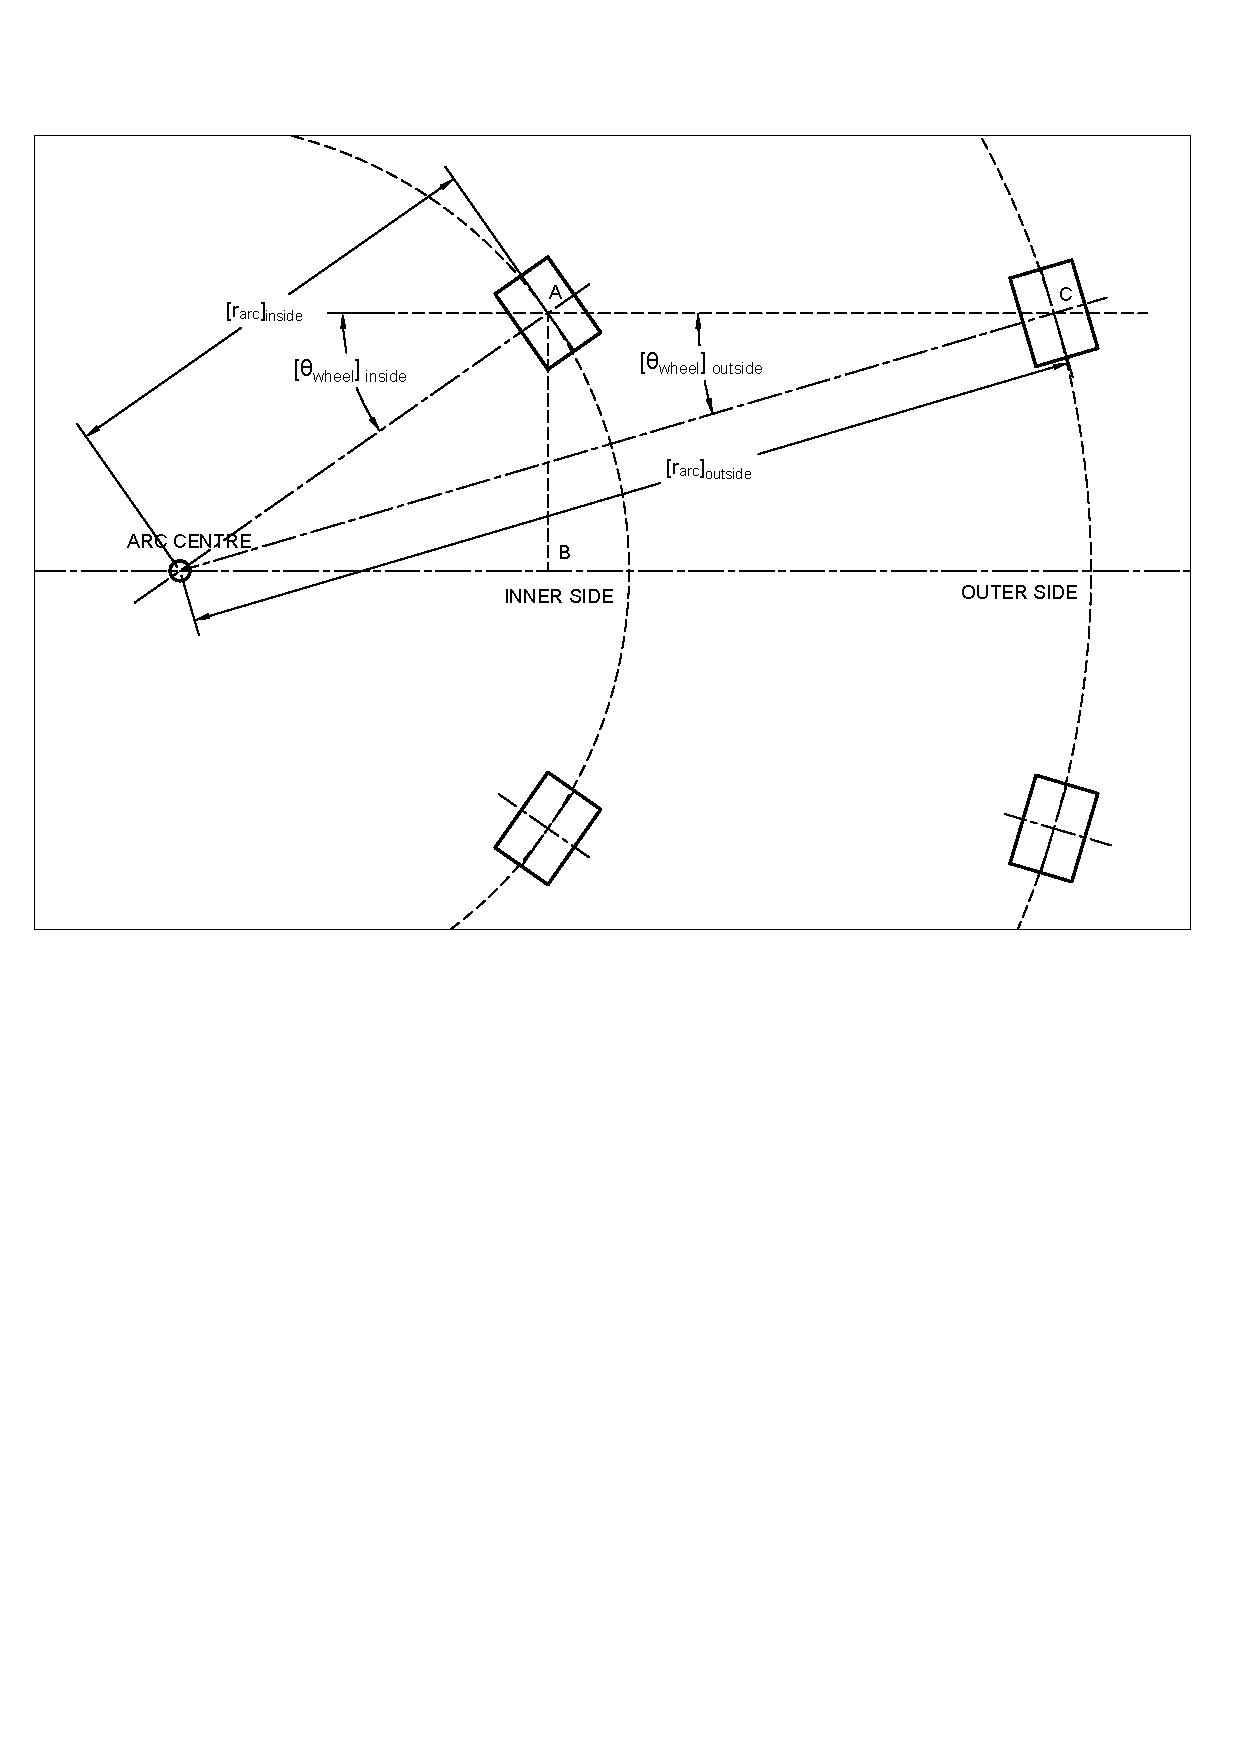
\includegraphics[clip, trim=1cm 14cm 1cm 3cm,width=1\linewidth]{figures/arcCalculations}
          \caption[Drawing of the front and rear wheels and the associated traversal arcs.]{Drawing of the front and rear wheels and the associated traversal arcs.}
          \label{fig:softDev-arcCalculations}
        \end{figure}
        
        The first angle, the angle of the front-inner wheel (relative to the direction of the arc; the closest side to the arc centre-point), was calculated by (\ref{eq:softDev-innerWheelAngle}) since it was known that the inner wheels would exhibit the greatest angular displacement.
        
        \begin{equation}
          \label{eq:softDev-innerWheelAngle}
          \left[\theta_{\text{wheel}}\right]_{\text{inside}} = a\times \left[\theta_{\text{wheel}}\right]_{\text{max}}
        \end{equation}
        
        \begin{flushright}
          where $\theta_{\text{wheel}}$ is the angle of a wheel and $a$ is the arc factor.
        \end{flushright}
        
        It was decided that the amount by which the centre wheels were offset from the centre of the rover, in the $x$ direction, was negligible (i.e. the wheels on each side of the suspension system were equally distributed) and so the rear wheels' angles were simply the same as those of the front wheels but in the opposite direction.
        
        Using $\left[\theta_{\text{wheel}}\right]_{\text{inside}}$, the radius of the circle formed by the inner-side wheels was calculated by (\ref{eq:softDev-innerWheelRadius}) and used to find the position of the centre-point of the circle which was representative of the centre-point of the arc of traversal of the rover. The circle made by the outer wheels shared this centre-point and the distance between the front wheels of each side of the suspension system was used to calculate the radius of the outer circle in (\ref{eq:softDev-outerWheelRadius}). Therefore, since the outer circle intersected with the outer wheels, the tangent at the points of intersection could be found by (\ref{eq:softDev-outerWheelAngle}) and this was the required angle of the outer wheels.
        
        \begin{equation}
          \label{eq:softDev-innerWheelRadius}
          \left[r_{\text{arc}}\right]_{\text{inside}} = \frac{\text{AB}}{\sin\left(\left[\theta_{\text{wheel}}\right]_{\text{inside}}\right)}
        \end{equation}
        \begin{flushright}
          where $\left[r_{\text{arc}}\right]_{\text{inside}}$ is the radius of the circle made by the inner side wheels.
        \end{flushright}
        
        \begin{equation}
          \label{eq:softDev-outerWheelRadius}
          \left[r_{\text{arc}}\right]_{\text{outside}} = \left[r_{\text{arc}}\right]_{\text{inside}} + \text{AC}
        \end{equation}
        \begin{flushright}
          where $\left[r_{\text{arc}}\right]_{\text{outside}}$ is the radius of the circle made by the outer side wheels.
        \end{flushright}
         
        \begin{equation}
          \label{eq:softDev-outerWheelAngle}
          \left[\theta_{\text{wheel}}\right]_{\text{outside}} = \arcsin\left(\frac{\text{AB}}{\left[r_{\text{arc}}\right]_{\text{outside}}}\right)
        \end{equation}
        
        The velocities were simply calculated by applying the velocity factor to the outer side wheels due to the fact that they were to traverse further, and scaling the factor down by the ratio of the two circle radii for the inner side wheels. The method used in the dispatch stage to perform the above calculations is included as Snippet~\ref{code:arcCalculationMethod}.
        
        \begin{code}
          \begin{minted}{js}
/**
 * Compute the arc dimensions of the wheels for a given arc factor
 * @param  {Number} arcFactor The factor by which the rover should turn/arc
 * @return {Object}           An object of the calculated dimensions
 */
function _computeArc(arcFactor) {
  const largeSide = (arcFactor < 0) ? 'Right' : 'Left';
  const smallSide = (largeSide === 'Right') ? 'Left' : 'Right';
  const smallAngle = arcFactor * 45;
  const smallRadius = config.hardware.wheelPitch / Math.sin(deg2rad(Math.abs(smallAngle)));
  const largeRadius = config.hardware.wheelSpan + smallRadius;
  const largeAngle = (arcFactor < 0 ? -1 : 1) * rad2deg(Math.asin(config.hardware.wheelPitch / largeRadius));

  return {
    largeSide,
    smallSide,
    smallAngle,
    smallRadius,
    largeRadius,
    largeAngle,
  };
}        		
          \end{minted}
          \caption{Method used to perform the arc calculations given a traversal arc factor.}
          \label{code:arcCalculationMethod}
        \end{code}
      
    \subsection{Socket.io Channels}
      The Socket.io channels used throughout the project is summarised in Table~\ref{tab:softDev-socketChannelResponsiblities} based on discussions thereof in the software design sections.
      
      \begin{table}[h!]
      \centering
      \begin{tabular}{@{}L{0.12\textwidth}L{0.15\textwidth}L{0.45\textwidth}L{0.2\textwidth}@{}}
      \toprule \textbf{Socket.io Channel} & \textbf{Applicable Software Components}                                    & \textbf{Description}                                                                                                                                                                                                                    & \textbf{Channel Data Responsibilities}                                                                                                                                                   \\ \midrule
      RCEIO             & \begin{tabular}[c]{@{}l@{}}RCE\\ RSVP Server\end{tabular}         & Serves as the only method of message data type communication between the RCE and the RSVP Server.                                                                                                                              & \begin{tabular}[c]{@{}L{0.2\textwidth}@{}}- Transmission of commands\\ - Transmission of telemetry\\ - Synchronisation of data stores\\ - Transport of custom requests\end{tabular}                    \\ \midrule
      KurentoIO         & \begin{tabular}[c]{@{}l@{}}RSVP Server\\ RSVP Client\end{tabular} & The signalling between the implementation of Kurento on the RSVP server and those on the connected RSVP Clients. Servers as the transport for SDP and ICE offers as well as other signalling events between the two endpoints. & \begin{tabular}[c]{@{}L{0.2\textwidth}@{}}- Transmission of SDP offers\\ - Transmission of ICE candidates\end{tabular}                                                                             \\ \midrule
      ControlIO         & \begin{tabular}[c]{@{}l@{}}RSVP Server\\ RSVP Client\end{tabular} & The first of the two message data specific channels between the RSVP Server and the RSVP Client. Handles control data and is restricted to only the client that is in control of the rover.                                    & \begin{tabular}[c]{@{}L{0.2\textwidth}@{}}- Transmission of RoSE commands\\ - Transmission of interactive control signals\\ - Transmission of other control related events and messages\end{tabular} \\ \midrule
      TeleIO            & \begin{tabular}[c]{@{}l@{}}RSVP Server\\ RSVP Client\end{tabular} & The second channel between the RSVP Server and the RSVP Client facilitating all types of telemetry.                                                                                                                            & \begin{tabular}[c]{@{}L{0.2\textwidth}@{}}- Transmission of telemetry data\\ - Synchronisation of data stores\end{tabular}                                                                         \\ \bottomrule
      \end{tabular}
      \caption{Table summarising the responsibilities of each of the implemented Socket.io channels.}
      \label{tab:softDev-socketChannelResponsiblities}
      \end{table}

      Each Socket.io endpoint component in the endpoint-translator pair included in initialisation method which registered the WebSocket channel and attached the required listeners to the instance. The listeners that were registered referenced handler methods exposed by the translator component keeping the endpoint component simple. The endpoint component also provided lower level methods for performing operations such as sending custom requests. Snippet~\ref{code:softDev-socketEndpointExample} includes an example endpoint implementation structure.
      
      \newpage
      \begin{code}
        \begin{minted}{js}
          import * as rceIOTranslator from './<channel>-translator'; // The translator associated with the socket channel
          import Socket from 'koa-socket'; // The Node.js module providing the Socket.io implementation for the server stack used in this particular software component
          
          const log = debug('rce:socket');
          
          let <channel>;
          
          /**
           * Initialise the socket instance and attach the associated handlers to it
           */
          export default function init() {
            // Instantiate the socket
            <channel> = new Socket('<channel>');
          
            // Listen on the `connection` event to detect a successful connection
            socket.on('connection', () => {
              store.rceState.set('<channel>.connected', true); // Update the store to reflect the new state of the connection
            });
            
            // Register the listeners associated with the channel, passing in references to the translator methods
            socket.on('data', <channel>Translator.onData);
            socket.on('post', <channel>Translator.onPost);
            socket.on('request', <channel>Translator.onRequest);
          }
          
          /**
           * Send a `request` type message via the socket, with a given payload
           * @param	{String}  type    The type of request
           * @param {Object}  payload	Payload to include with the message
           *
           * This is an example of a custom low level operation included in the endpoint API
           */
          export function sendRequest(type, payload) {
            <channel>.broadcast('request', { type, payload });
          }
          
        \end{minted}
        \caption{An example Socket.io endpoint file where \mintinline{js}{<channel>} is the name of the channel.}
        \label{code:softDev-socketEndpointExample}
      \end{code}
    
    \subsection{RCE Video Streaming Utility}
      A candidate solution to the video streaming on the RCE software component was to use the Linux tool \mintinline{js}{Video4Linux2} (\mintinline{js}{v4l2}) which allowed streaming of video in realtime from hardware available to the operating system, including devices of the UVC driver-less class. Another tool, \mintinline{js}{ffmpeg}, which leveraged \mintinline{js}{v4l2} for video capture, allowed the creation of an HTTP and RTSP server which could be connected to from an external endpoint on the network. However, tests performed with an \mintinline{js}{ffmepg} implementation proved the tool unsuitable for the project due to low reliability and high CPU cost. Yet another utility was found, \mintinline{js}{mjpeg-streamer}, which was also tested and found to be a well performing and reliable alternative to \mintinline{js}{ffmpeg}. \mintinline{js}{mjpeg-streamer} provided streaming of the video data in one command line (Snippet~\ref{code:mjpeg-streamerCmdLine}), which was spawned as a child process by the RCE as in Snippet~\ref{code:mjpeg-streamerChildProcess}.
      
      \begin{code}
        \begin{minted}{js}
'/usr/local/bin/mjpg_streamer -i "/usr/local/lib/input_uvc.so -d /dev/video0 -n -r 640x480 -f 30" -o "/usr/local/lib//output_http.so -n -p 8080 -w /usr/local/www"'
        \end{minted}
        \caption{The \mintinline{js}{bash} command which was executed to invoke \mintinline{js}{mjpeg-streamer} and stream the video data via the specified port.}
        \label{code:mjpeg-streamerCmdLine}
      \end{code}
      
      \begin{code}
        \begin{minted}{js}
          import child from 'child_process'; // A Node.js provide API for spawning additional processes outside that of the Node.js program
          
          // Spawn the camera process
          camProcess = child.exec(config.hardware.cameraStartCmdLine, (err) => {
            // Errors handled here
          });
        \end{minted}
        \caption{Snippet showing the spawning of a child process in which \mintinline{js}{mjpeg-streamer} was invoked.}
        \label{code:mjpeg-streamerChildProcess}
      \end{code}
      
      